\chapter{Introduction}
There are vast amount of information and products available on the web. Even within a single websites the number of items can be overwhelming for users. Examples of sites where this applies are news sites, streaming services, and e-commerce sites. Recommender systems can help creating a better user experience by helping users find what they are looking for and are interested in. They can also help businesses in different ways, like showing targeted ads or help offering a better product.\\

In this paper, we will explore recommender systems, specifically session-based recommender systems. We will look at the use of deep learning and recurrent neural networks(RNN) for this, as compared to classical methods.\\

This introduction chapter introduces session-based recommender systems, some of the challenges in the domain, recurrent neural networks and how they fit into the problem.
The second chapter, State of the art, looks at different methods that exist, but focuses on what has been done in terms of deep learning and RNNs.
In the third chapter, Core, we explain our own work.
Our experiments and results are laid out in the fourth chapter, Experiments and results.
Lastly follows a the conclusion and further work, which summarize what has been done, which challenges remain and needs to be studied further.

%----------------------------
%Give short introduction about what this report will discuss (rnn), touch very briefly upon what the reader should have in mind and can expect from the report. Explain what will be discussed in the different chapters.
%
%Touch very briefly upon what rnn is, so that the reader understands enough to understand the next sections, before we get to background. (Or should background come before motivation and objectives of work?)


\section{Motivation}
\label{sec:motivation}

As mentioned, recommender systems can help both users looking for content and the providers of the content. Users are generally interested in finding what they are looking for as easy as possible, or to be shown products or content that interests them, but which they normally would not have discovered on their own. Spotify helps users discover new content introducing them to new music, tailored to the user, through their Discover Weekly\cite{discover-weekly} playlists. When a user buys something on an e-commerce site like Amazon, the site display items to the user, that other users bought together with the original item. These are examples where recommender systems helps users discover new content and helps user find products they are interested in.\\

For the provider, or seller, there may be different reasons to use recommender systems depending on their business model. Google earn money when users click on ads, so it is important for them to show relevant ads with high probability of getting clicked by the user. Similarly, YouTube earns money by showing commercials in their videos, and thus they can earn more money by making the user watch more videos. This can be accomplished by suggesting videos that the user wants to watch. Or like in the Amazon example, suggesting additional items might make the buyer but more than he had initially intended. Recommender systems are also used by Facebook and news feeds which tries to filter out what is shown to the user.\\

%Why are recommender systems interesting? (interesting for both users and provider/seller) occour in many situations, especially on the web, ads placement on sites like google and finn.no, music on spotify, movies on netflix, media content on youtube, any webshop what so ever, facebook...

In the examples above, recommendations are made based on the user profile, which has information about the user interests. This profile is built up over time, as the user interacts with a system/site. Or in the Amazon example, the recommendation may only be based on a single or few items that the user bought. To make good recommendations in these scenarios, it is assumed that one has access to a user profile, but this might not always be the case. Multiple users may share an account, maybe the user is new, or maybe the user is not logged in at all. Sites can use cookies to get some historical data about the user when he is not logged in, but this is not very reliable either. There might not exist any cookies because the user is completely new to the site, or he may have deleted them. And even though we have access to cookies with information, the traffic might come from a computer shared by family members for example. Son and mom are probably not buying the same clothes, or listening to the same music. But even when we assume that it is possible to know who the user is, and what his interests are, he might be searching for content/products that is not related to his interests at all. An example of this could be a professional angler that wants to buy beginner equipment for his nephew, or maybe the angler suddenly has decided to start playing football and is looking for football equipment. Another example is a programmer who wants to listen to calm classical music while he works, but when he goes to the gym after work, he wants to listen to energetic techno. In these situations the recommender system will not be able to make good recommendations based on what it knows about the user. Only the current session might be relevant to what the user is looking for.\\

%Why are they interesting in the session-based setting? (don't have user profile, don't know what the user likes, still want to give good recommendations. Would be nice if we could do better than just recommending generally popular or similar items)
%Maybe different users use the same account (netflix), or the traffic comes from a family computer where different family members have very different interests.
%Even a single user may have vastly different interest from time to time. A user may look for different things depending on holidays or events, and he might be looking for different things during and after work hours. Also, especially in the case of shopping, a user might be looking for items not related to his interest at all, so the only info we have for recommendation is the current session. 

Recurrent neural networks intuitively fits well as a recommender system, especially in the session-based scenario. They do not suffer from the cold start scenario, they can perform well with minimal information about items, and they make it easier to extract good features \cite{ZALANDO:understanding-consumer-histories}. Also, RNNs does not suffer from some of the assumptions that classical neural networks do. With recent advances in architectures for RNN, ways to circumvent training problems, and better hardware, RNNs have become very feasible to use. Much research has been done on RNNs recently, some of this research focuses on using RNN as a session-based recommender system. The results are promising, and it seems like RNNs are fully capable of competing with state of the art recommender systems.

%Why are RNN interesting? with invention of the LSTM and GRU units, combined with better hardware, they have become much more feasible to use

%RNNs have properties that intuitively fits in a recommender system, and maybe moreso in the session-based variant.

%RNN does not suffer from the cold start scenario, makes it easier to extract good features, and can even perform well with no information about items.


%---------------------------
%Why are RNNs interesting?
%- easier feature extraction/engineering (zalando blog)
%- the model fits very well with problems involving sequences. can model sequences, has memory
%- has achieved very promising and state of the are results 
%- has recently become interesting because of lstm, gru which helps with vanishing and exploding gradients, pluss powerful hardware
%- does not suffer from cold-start problem. can apply on unknown users
%- can easily work with sequences of different length

\section{Objectives}
The goal of this paper and the work described in it, is to implement an RNN and test how it performs as a recommender system. We explore recommender systems, particularly those that deal with session-based recommendation. Specifically we look at the use of RNNs as session-based recommender systems. We want to know if they can compete with other models currently in use. Furthermore, we look at different architectures and ways of optimizing them to improve results. Our work is inspired, mainly, by the work in \cite{DBLP:journals/corr/HidasiKBT15} and \cite{DBLP:journals/corr/LiuWWL016}. The first paper explores the use of an RNN for session-based recommendations compared to other methods. The second paper explores how adding context information as input to the network can improve the results.


%implement an rnn and test its performance as a recommender system.
%explore recommender systems, specifically session based. Explore the use of using rnn for this instead of classical methods. The work is inspired by paper x, y, z, and these are used as a basis for our exploration. 

%-----------------------

%- look at work that has been done, state of the art
%- look at how results can be improved when predicting sequences
%- specifically interested in situations that apply to online users where we might have no prior knowledge of the user

\section{Background}
In this section we explain, on a high level, terms and concepts used in this paper.

\subsection{Recommender systems}
As touched upon in \ref{sec:motivation}, recommender systems are systems that try to predict a users evaluation of an item, or what items a user is interested in interacting with. They can be, and are, used in many areas. Some examples are music, movies, news, restaurants, recipes, online shopping, and dating. Figure \ref{fig:recsys-example-xbox} shows an example of recommendations made by Amazon and YouTube when looking at a Xbox One.\\
	
\begin{figure}[htp]
	\centering
	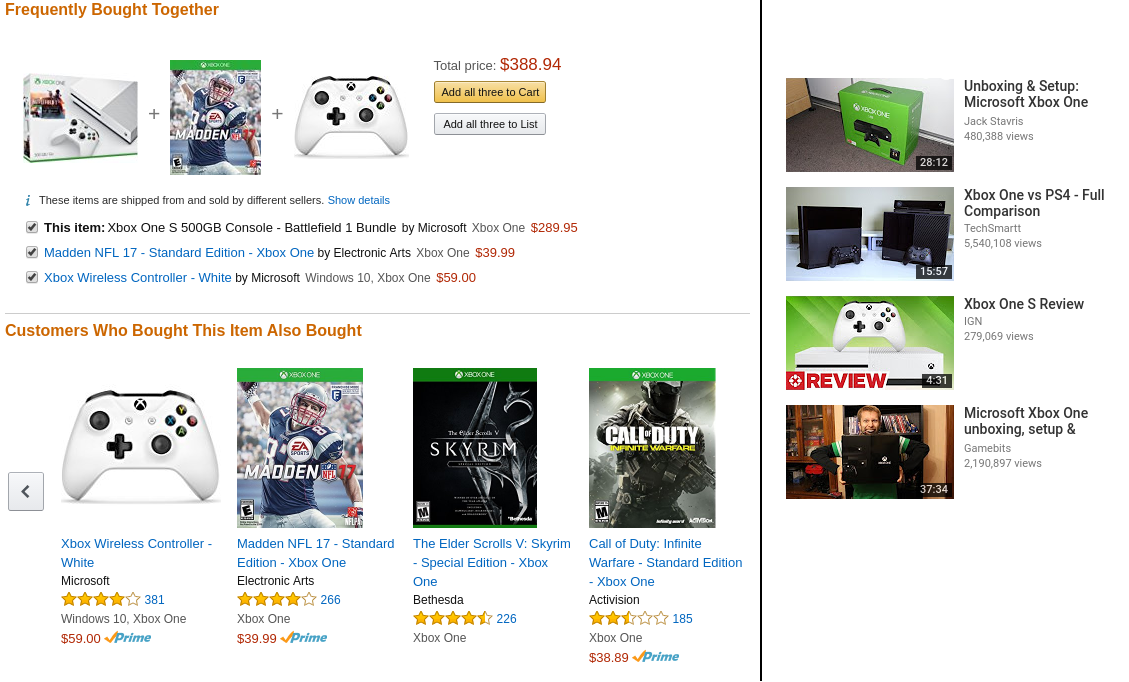
\includegraphics[width=1.1\textwidth]{fig/recsys_example_xbox.png}
	\caption{Recommendations from Amazon (left) and YouTube (right) when looking at Xbox One.}
	\label{fig:recsys-example-xbox}
\end{figure}

Note that there is a subtle difference between predicting which items a user will like, and which items he is interested in interacting with. The former case involves predicting what rating a user will give a movie or whether a user is likely to purchase one or any item. On the other hand, the latter case does not worry about how the user will interact with an item, but whether the user will choose to interact with the item, given the choice. To exemplify this, lets look at a movie streaming site. Should the site recommend movies that the user will rate highly if he watches them, or should it recommend movies that the user is likely to watch independent of how he will rate it? The answer will probably depend on the business and other factors, the point is that there is a difference between the two approaches. In the movie example, it is reasonable to think that how a user would rate a movie is less dynamic than what he want to watch. His ratings would probably depend a lot on his personal preferences, which usually change slowly over time. What he is interested in watching at any point, however, might depend more on circumstances. This was illustrated earlier with the worker who wanted to listen to different genres at during work and his workout session.\\

It is therefore clear that the goal of recommender systems may vary with different businesses and settings. In this paper we are mainly concerned with predicting the next item the user will choose to interact with.\\

There are two classical approaches to recommender systems, collaborative filtering and content-based filtering. These two methods can be combined into a hybrid approach.

\subsection{Collaborative filtering}
Collaborative filtering uses information about users preferences to recommend items highly rated by similar users. To illustrate, let us look at a movie recommendation system. A user log into a website where he can rate movies he has seen and the site recommends movies to the user based on his ratings. With the collaborative filtering approach, the user needs to rate some movies to get good recommendations, and as the user rate more and more movies he has seen, the system is able to make better recommendations. To make the recommendations, the system groups together similar users. A user is then recommended movies that he has not seen and that was rated highly by other similar users. The system decides whether users are similar by looking at how like-minded they are, that is, how similar they rate movies. This is illustrated in figure \ref{fig:collaborative-filtering}. The system predicts what rating the question mark will be by guessing the same rating as given by similar users (highlighted in green).

\begin{figure}[htp]
	\centering
	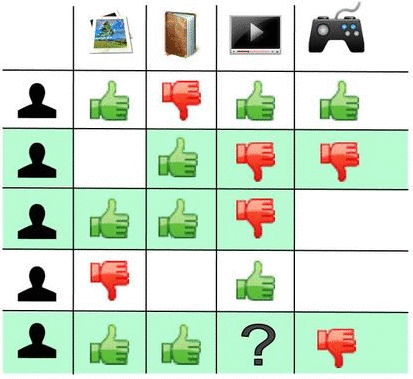
\includegraphics[width=0.4\textwidth]{fig/collab-filtering.png}
	\caption{Illustration of collaborative filtering}
	\source{https://en.wikipedia.org/wiki/Collaborative\_filtering\#/media/File:Collaborative\_filtering.gif}
	\label{fig:collaborative-filtering}
\end{figure}

\subsection{Session-based recommender systems}
Session-based recommender systems tries to do predictions mostly based on the current user session. Sessions are often limited in time, and, as we have seen, the users interests might vary between sessions. Generally we no information about the user, and since the sessions are short, we do not get much information either. There may be many reasons for this lack of information. Some examples are new users, users sharing accounts, and small e-commerce sites where each unique user only visits it a couple of times. Furthermore, even though we have access to information about the users interest, this might be of minimal use if the users interests vary greatly between sessions. A session usually consists of multiple user actions on a number of items, in the order the actions happen, constrained to a short timespan. What ''short timespan'' means will depend on the domain, but is often on the scale of minutes.\\


%theoretical background. explain everything at a high level (more technical explanations can be done in state of the art). Everything that is used in the core

%- What is a recommender system?
%   Why do recommender systems exist
%   Two sligthly different types of recommender systems (predict what the user will give a good rating, and predict what the user would want to interact with independently of whether he will give it a good rating or not)
%- What is a session-based recommender system?
%- What is a neural network
%- What is deep learning
%- What is RNN
%- GRU and LSTM
%- Contextualise what I am doing
%- what is contextual information (external [time, weather, ...] and item specific context [more info abiout the item: image, text, category...])

%-----------------------
%- explain the problem domain
%- explain rnn